\documentclass[6008notes.tex]{subfiles}
\begin{document}
\graphicspath{ {images/measrand/} }

\section{Measuring Randomness}

\subsection{Introduction to Information-Theoretic Measures of Randomness}

We just saw some basics for decision making under uncertainty and expected values of random variables. One way we saw for measuring uncertainty was variance. Now we look at a different way of measuring uncertainty or randomness using some ideas from information theory.

In this section, we answer the following questions in terms of bits (as in bits on a computer; everything stored on a computer is actually 0's and 1's each of which is 1 bit):

\begin{itemize}
\item How do we measure how random an event is?

\item How do we measure how random a random variable or a distribution is?

\item How do we measure how different two distributions are?

\item How much information do two random variables share?
\end{itemize}

For now, this material may seem like a bizarre exercise relating to expectation of random variables, but as we will see in the third part of the course on learning probabilistic models, information theory provides perhaps the cleanest derivations for some of the learning algorithms we will derive!

More broadly but beyond the scope of 6.008.1x, information theory is often used to show what the best possible performance we should even hope an inference algorithm can achieve such as fundamental limits to how accurate we can make a prediction. And if you can show that your inference algorithm's performance meets the fundamental limit, then that certifies that your inference algorithm is optimal! Inference and information theory are heavily intertwined!

\subsection{Shannon Information Content}

First, let's consider storing an integer that isn't random. Let's say we have an integer that is from $0,1,\dots ,63$. Then the number of bits needed to store this integer is $log_2?(64)=6$ bits: you tell me 6 bits and I can tell you exactly what the integer is.

A different way to think about this result is that we don't \textit{a priori} know which of the 64 outcomes is going to be stored, and so each outcome is equally likely with probability $\frac{1}{64}$. Then the number of bits needed to store an event $\mathcal{A}$ is given by what's called the ``Shannon information content'' (also called self-information):

{\centering$\log _{2}\frac{1}{\mathbb {P}(\mathcal{A})}.$ \par}

In particular, for an integer $x\in \{ 0,1,\dots ,63\}$, the Shannon information content of observing $x$ is

{\centering$\log _{2}\frac{1}{\mathbb {P}(\text {integer is }x)}=\log _{2}\frac{1}{1/64}=\log _{2}64=6\text { bits}.$ \par}
 
If instead, the integer was deterministically 0 and never equal to any of the other values $0,1,\dots ,63$, then the Shannon information content of observing integer 0 is

{\centering$\log _{2}\frac{1}{\mathbb {P}(\text {integer is }0)}=\log _{2}\frac{1}{1}=0\text { bits}.$ \par}

This is not surprising in that a outcome that we deterministically always observe tells us no new information. Meanwhile, for each integer $x\in \{ 0,1,\dots ,63\}$,

{\centering$\log _{2}\frac{1}{\mathbb {P}(\text {integer is }x)}=\log _{2}\frac{1}{0}=\infty \text { bits}.$ \par}
 
How could observing one of the integers \{ 1,2,\dots ,63\} tell us infinite bits of information?! Well, this isn't an issue since the event that we observe any of these integers has probability 0 and is thus impossible. An interpration of Shannon information content is how surprised we would be to observe an event. In this sense, observing an impossible event would be infinitely surprising.

It is possible to have the Shannon information content of an event be some fractional number of bits (e.g., 0.7 bits). The interpretation is that from many repeats of the underlying experiment, the average number of bits needed to store the event is given by the Shannon information content, which can be fractional.

\subsection{Shannon Entropy}

To go from the number of bits contained in an event to the number of bits contained in a random variable, we simply take the expectation of the Shannon information content across the possible outcomes. The resulting quantity is called the entropy of a random variable:

{\centering$H(X)=\sum _{x}p_{X}(x)\underbrace{\log _{2}\frac{1}{p_{X}(x)}}_{\text {Shannon information content of event }X=x}.$ \par}
 
The interpretation is that on average, the number of bits needed to encode each i.i.d. sample of a random variable $X$ is $H(X)$. In fact, if we sample $n$ times i.i.d. from $p_X$, then two fundamental results in information theory that are beyond the scope of this course state that: (a) there's an algorithm that is able to store these $n$ samples in $nH(X)$ bits, and (b) we can't possibly store the sequence in fewer than $nH(X)$ bits!

Example: If $X$ is a fair coin toss ``heads'' or ``tails'' each with probability 1/2, then

\begin{eqnarray*}
H(X)
&=& p_X(\text{heads}) \log_2 \frac1{p_X(\text{heads})}
+ p_X(\text{tails}) \log_2 \frac1{p_X(\text{tails})} \\
&=& \frac12 \cdot \underbrace{\log_2 \frac1{\frac{1}{2}}}_1
+ \frac12 \cdot \underbrace{\log_2 \frac1{\frac{1}{2}}}_1 \\
&=& 1 \text{ bit}.
\end{eqnarray*}
 
Example: If $X$ is a biased coin toss where heads occurs with probability 1 then

\begin{eqnarray*}
H(X)
&=& p_X(\text{heads}) \log_2 \frac1{p_X(\text{heads})}
+ p_X(\text{tails}) \log_2 \frac1{p_X(\text{tails})} \\
&=& 1 \cdot \underbrace{\log_2 \frac11}_0
+ 0 \cdot \cdot \underbrace{\log_2 \frac10}_1 \\
&=& 0 \text{ bits},
\end{eqnarray*}
 
where $0 \log _2 \frac10 = 0 \log _2 1 - 0 \log _2 0 = 0$ using the convention that $0 \log _2 0 \triangleq 0$. (Note: You can use l'Hopital's rule from calculus to show that $\lim _{x\rightarrow 0} x \log x = 0$ and $\lim _{x\rightarrow 0} x \log \frac1x = 0$.)

\paragraph{Notation:} Note that entropy $H(X) = \sum _ x p_ X(x) \log _2 \frac{1}{p_ X(x)}$ is in the form of an expectation! So in fact, we can write an expectation:

{\centering$H(X) = \mathbb {E}\Big[\log _2 \frac{1}{p_ X(X)}\Big].$ \par}
 
\subsection{Information Divergence}

Information divergence (also called ``Kullback-Leibler divergence'' or ``KL divergence'' for short, or also ``relative entropy'') is a measure of how different two distributions $p$ and $q$ (over the same alphabet) are. To come up with information divergence, first, note that entropy of a random variable with distribution $p$ could be thought of as the expected number of bits needed to encode a sample from $p$ using the information content according to distribution $p$:

{\centering$\underbrace{\sum _{x}p(x)}_{\text {expectation using }p}\underbrace{\log _{2}\frac{1}{p(x)}}_{\text {information content according to }p}\triangleq \mathbb {E}_{X \sim p}\Big[\log _{2}\frac{1}{p(X)}\Big].$ \par}
 
Here, we have introduced a new notation: $\mathbb {E}_{X \sim p}$ means that we are taking the expectation with respect to random variable $X$ drawn from the distribution $p$. If it's clear which random variable we are taking the expectation with respect to, we will often just abbreviate the notation and write $\mathbb {E}_{p}$ instead of $\mathbb {E}_{X \sim p}$.

If instead we look at the information content according to a different distribution $q$, we get

{\centering$\underbrace{\sum _{x}p(x)}_{\text {expectation using }p}\underbrace{\log _{2}\frac{1}{q(x)}}_{\text {information content according to }q}\triangleq \mathbb {E}_{X \sim p}\Big[\log _{2}\frac{1}{q(X)}\Big].$ \par}
 
It turns out that if we are actually sampling from $p$ but encoding samples as if they were from a different distribution $q$, then we always need to use more bits! This isn't terribly surprising in light of the fundamental result we alluded to that entropy of a random variable with distribution $p$ is the minimum number of bits needed to encode samples from $p$.

Information divergence is the price you pay in bits for trying to encode a sample from $p$ using information content according to $q$ instead of according to $p$:

{\centering$D(p\parallel q)=\mathbb {E}_{X \sim p}\Big[\log _{2}\frac{1}{q(X)}\Big]-\mathbb {E}_{X \sim p}\Big[\log _{2}\frac{1}{p(X)}\Big].$ \par}
 
Information divergence is always at least 0, and when it is equal to 0, then this means that $p$ and $q$are the same distribution (i.e., $p(x)=q(x)$ for all $x$). This property is called Gibbs' inequality.

Gibbs' inequality makes information divergence seem a bit like a distance. However, information divergence is not like a distance in that it is not symmetric: in general, $D(p \parallel q) \ne D(q \parallel p)$.

Often times, the equation for information divergence is written more concisely as

{\centering$D(p\parallel q) = \sum _ x p(x) \log \frac{p(x)}{q(x)},$ \par}
 
which you can get as follows:

\begin{eqnarray*}
D(p\parallel q)
&=&
  \mathbb{E}_{X \sim p}\Big[\log_{2}\frac{1}{q(X)}\Big]
- \mathbb{E}_{X \sim p}\Big[\log_{2}\frac{1}{p(X)}\Big] \\
&=&
  \sum_x p(x) \log_2 \frac{1}{q(x)}
- \sum_x p(x) \log_2 \frac{1}{p(x)} \\
&=&
  \sum_x p(x)
  \Big[ \log_2 \frac{1}{q(x)} - \log_2 \frac{1}{p(x)} \Big] \\
&=&
  \sum_x p(x)
  \log_2 \frac{p(x)}{q(x)}.
\end{eqnarray*}

Meanwhile, suppose $q$ is a distribution for a biased coin that always comes up heads (perhaps it's double-headed):

\begin{eqnarray*}
q(x)
&=&
\begin{cases}
1 & \text{if }x=\text{heads}, \\
0 & \text{if }x=\text{tails}. \\
\end{cases}
\end{eqnarray*}

Then

\begin{eqnarray*}
D(p \parallel q)
&=&
  p(\text{heads}) \log_2 \frac{p(\text{heads})}{q(\text{heads})}
+ p(\text{tails}) \log_2 \frac{p(\text{tails})}{q(\text{tails})} \\
&=&
  \frac12\log_2 \frac{\frac12}1
+ \underbrace{\frac12\log_2 \frac{\frac12}0}_{\infty} \\
&=&
  \infty\text{ bits}.
\end{eqnarray*}

This is not surprising: If we are sampling from $p$ (for which we could get tails) but trying to encode the sample using $q$ (which cannot possibly encode tails), then if we get tails, we are stuck: we can't store it! This incurs a penalty of infinity bits.

Meanwhile,

\begin{eqnarray*}
D(q \parallel p)
&=&
  q(\text{heads}) \log_2 \frac{q(\text{heads})}{p(\text{heads})}
+ q(\text{tails}) \log_2 \frac{q(\text{tails})}{p(\text{tails})} \\
&=&
  1 \log_2 \frac1{\frac12}
+ \underbrace{0 \log_2 \frac0{\frac12}}_0 \\
&=&
  1\text{ bit}.
\end{eqnarray*}

When we sample from $q$, we always get heads. In fact, as we saw previously, the entropy of the distribution for an always-heads coin flip is 0 bits since there's no randomness. But here we are sampling from $q$ and storing the sample using distribution $p$. For a fair coin flip, encoding using distribution $p$ would store each sample using on average 1 bit. Thus, even though a sample from $q$ is deterministically heads, we store it using 1 bit. This is the penalty we pay for storing a sample from $q$ using distribution $p$.

Notice that in this example, $D(p \parallel q) \ne D(q \parallel p)$. They aren't even close --- one is infinity and the other is finite!

\subsection{Proof of Gibbs' Inequality}

We provide a proof for Gibbs' inequality here for those who are interested. For those of you up for the challenge, try to prove it yourself!

There are various ways to prove Gibbs' inequality. We'll be using a way that relies on the fact that $\ln x\le x-1$ for all $x>0$, with equality if and only if $x=1$, which we provide a proof for at the end of this page, but for which you can also readily see from the following plot:

{\centering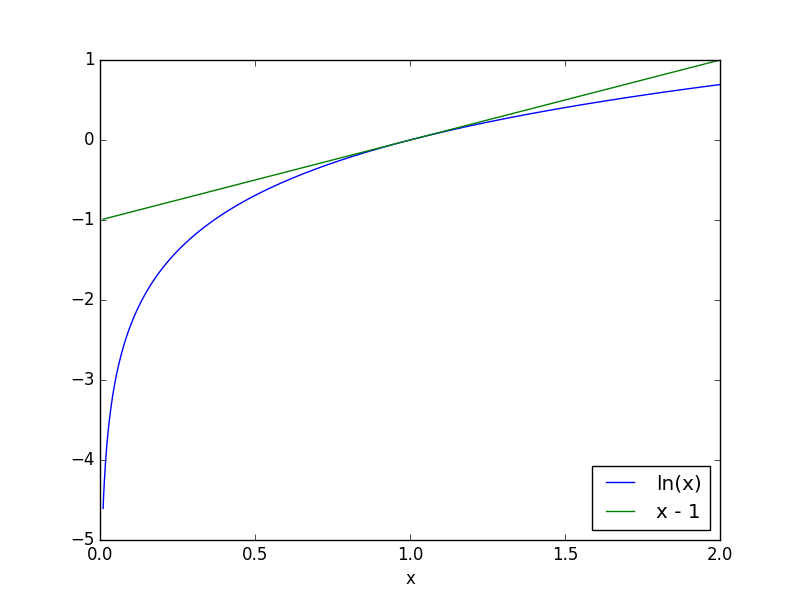
\includegraphics[scale=0.4]{images_sec-gibbs-inequality-helper} \par}

Code for producing this plot is also at the end of this section.

\paragraph{Gibbs' inequality:} For any two distributions $p$ and $q$ defined over the same alphabet, we have $D(p\parallel q)\ge 0$, where equality holds if and only if $p$ and $q$ are the same distribution, i.e., $p(x)=q(x)$ for all $x$.

\paragraph{Proof:} Recall that changing the base of a log just changes the log by a constant factor:

{\centering$\log _{2}x=\frac{\ln x}{\ln 2}.$ \par}

Let $\mathcal{X}$ be the alphabet of distribution $p$ restricted to where the probability is positive, i.e., $\mathcal{X}=\{ a\text { such that }p(a)>0\}$. (There is no need to look at values $a$ for which $p(a)=0$.)

If $q(a)=0$ for any $a\in \mathcal{X}$, then $D(p\parallel q)=\infty$, so trivially $D(p\parallel q)>0$.

What's left to consider is when $q(a)>0$ for every $a\in \mathcal{X}$. Then

{\renewcommand{\arraystretch}{1.5}
\begin{tabular}{l l l}
$D(p\parallel q)$ & $=$ & $\sum _{a\in \mathcal{X}}p(a)\log _{2}\frac{p(a)}{q(a)}$ \\
  & $=$ & $\frac{1}{\ln 2}\sum _{a\in \mathcal{X}}p(a)\ln \frac{p(a)}{q(a)}$ \\
  & $=$ & $-\frac{1}{\ln 2}\sum _{a\in \mathcal{X}}p(a)\ln \frac{q(a)}{p(a)}.$ 
\end{tabular}}
		
Next, using the fact that $\ln x\le x-1$ for all $x>0$, and accounting for the minus sign outside the summation,

{\renewcommand{\arraystretch}{1.5}
\begin{tabular}{l l l}
$D(p\parallel q)$ & $=$ & $-\frac{1}{\ln 2}\sum _{a\in \mathcal{X}}p(a)\ln \frac{q(a)}{p(a)}$ \\
  & $=$ & $-\frac{1}{\ln 2}\sum _{a\in \mathcal{X}}p(a)\Big(\frac{q(a)}{p(a)}-1\Big)$ \\
  & $=$ & $-\frac{1}{\ln 2}\sum _{a\in \mathcal{X}}\big (q(a)-p(a)\big )$ \\
  & $=$ & $-\frac{1}{\ln 2}\big (\underbrace{\sum _{a\in \mathcal{X}}q(a)}_{1}-\underbrace{\sum _{a\in \mathcal{X}}p(a)}_{1}\big )$ \\
  & $=$ & $0$ 
\end{tabular}}
			
Recall that inequality $\ln x\le x-1$ becomes an equality if and only if $x=1$. Thus, the inequality above becomes an equality if and only if, for all $a\in \mathcal{X}$, we have $\ln \frac{q(a)}{p(a)}=\frac{q(a)}{p(a)}-1$, which holds if and only if $\frac{q(a)}{p(a)}=1$. Thus $D(p\parallel q)=0$ if and only if $p(a)=q(a)$ for all $a\in \mathcal{X}$. This finishes the proof. $\square$

\paragraph{Claim:} $\ln x\le x-1$ for all $x>0$ where equality holds if and only if $x=1$.

\paragraph{Proof:} We show that the function $f$ given by $f(x)=x?1?\ln x$ is always at least 0 and achieves its minimum value at $x=1$. First, note that $f$ is differentiable for all $x>0$ (which implies that $f$ is continuous on $(0,\infty)$ and doesn't, for example, do some crazy jump midway through). In fact, the derivative of $f$ is given by

{\centering$\frac{d}{dx}f(x)=\frac{d}{dx}(x-1-\ln x)=1-\frac{1}{x}.$ \par}
 
On the interval $x>0$, the derivative is 0 (and so there's a local extremum) precisely when $x=1$. The question is whether this is a local minimum or a local maximum. We look at the second derivative of $f$ to do a second derivative test:

{\centering$\frac{d^{2}}{dx^{2}}f(x)=\frac{1}{x^{2}},$ \par}

which is strictly positive for all $x>0$. In other words, $x=1$ is a local minimum. The only possible other extrema could happen at the boundaries, but it's easy to check that

{\centering$\lim _{x\rightarrow 0}f(x) = \lim _{x\rightarrow 0} (x - 1 - \ln x) = -1 - \underbrace{\lim _{x\rightarrow 0} \ln x}_{-\infty } = \infty ,$ \par}

and

{\centering$\lim _{x\rightarrow \infty }f(x) = \lim _{x\rightarrow \infty } (x - 1 - \ln x) = \infty ,$ \par}

since $x$ grows faster than $\ln x$.

Hence, $f$ attains its global minimum at $x=1$, for which we have

{\centering$f(1)=1-1-\ln 1=0.$ \par}

Since this is the global minimum, we know that $f(x) \ge 0$ for all $x>0$. Furthermore, since there is only one unique global minimum $x=1$, we further conclude that $f(x)=0$ if and only if $x=1$. $\square$

\textbf{Code to produce the plot at the top of this section:}

\begin{lstlisting}
plt.figure()
plt.plot(x, np.log(x))
plt.plot(x, x - 1)
plt.xlabel('x')
plt.legend(['ln(x)', 'x - 1'], loc=4)
plt.show()
\end{lstlisting}

\subsection{Mutual Information}

Mutual information: For two discrete random variables $X$ and $Y$, the mutual information between $X$ and $Y$, denoted as $I(X;Y)$, measures how many much information they share. Specifically,

{\centering$I(X;Y)\triangleq D(p_{X,Y}\parallel p_{X}p_{Y}),$ \par}
 
where $p_Xp_Y$ is the distribution we get if $X$ and $Y$ were actually independent (i.e., if $X$ and $Y$ were actually independent, then we know that the joint probability table would satisfy $\mathbb {P}(X=x,Y=y)=p_{X}(x)p_{Y}(y)$.

The mutual information could be thought of as how far $X$ and $Y$ are from being independent, since if indeed they were independent, then $I(X;Y)=0$.

On the opposite extreme, consider when $X=Y$. Then we would expect $X$ and $Y$ to share the most possible amount of information. In this scenario, we can write $p_{X,Y}(x,y)=p_{X}(x)\mathbf{1}\{ x=y\}$, and so

\begin{eqnarray*}
I(X;Y)
&=&D(p_{X,Y}\parallel p_{X}p_{Y})\\
&=&\sum_{x}\sum_{y}p_{X,Y}(x,y)\log_{2}\frac{1}{p_{X}(x)p_{Y}(y)}\\
&&\quad
  -\sum_{x}\sum_{y}p_{X,Y}(x,y)\log_{2}\frac{1}{p_{X,Y}(x,y)}\\
&=&\sum_{x}\sum_{y}p_{X}(x)\mathbf{1}\{x=y\}\log_{2}\frac{1}{p_{X}(x)p_{Y}(y)}\\
&&\quad
  -\sum_{x}\sum_{y}p_{X}(x)\mathbf{1}\{x=y\}\log_{2}\frac{1}{p_{X}(x)\mathbf{1}\{x=y\}}\\
&=&\sum_{x}p_{X}(x)\log_{2}\Big(\frac{1}{p_{X}(x)}\Big)^{2}-\sum_{x}p_{X}(x)\log_{2}\frac{1}{p_{X}(x)}\\
&=&2\sum_{x}p_{X}(x)\log_{2}\frac{1}{p_{X}(x)}-\sum_{x}p_{X}(x)\log_{2}\frac{1}{p_{X}(x)}\\
&=&\sum_{x}p_{X}(x)\log_{2}\frac{1}{p_{X}(x)}\\
&=&H(X).
\end{eqnarray*}

This is not surprising: if $X$ and $Y$ are the same, then the number of bits they share is exactly the average number of bits needed to store $X$ (or $Y$), namely $H(X)$ bits.

\subsection{Exercise: Mutual Information}

Consider the following joint probability table for random variables $X$ and $Y$. We'll compute the mutual information $I(X;Y)$ of random variables $X$ and $Y$ step-by-step.

{\centering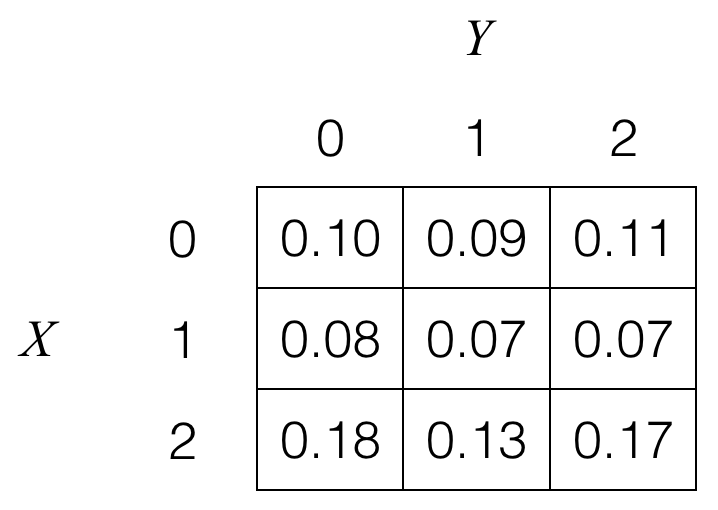
\includegraphics[scale=0.4]{images_sec-mutual-info-ex} \par}

Mutual information is about comparing the joint distribution of $X$ and $Y$ with what the joint distribution would be if $X$ and $Y$ were actually independent.

In Python (where we won't explicitly store the labels of the rows and columns):

\begin{lstlisting}
import numpy as np
joint_prob_XY = np.array([[0.10, 0.09, 0.11], [0.08, 0.07, 0.07], [0.18, 0.13, 0.17]])
\end{lstlisting}

The marginal distributions $p_X$ and $p_Y$ are given by:

\begin{lstlisting}
prob_X = joint_prob_XY.sum(axis=1)
prob_Y = joint_prob_XY.sum(axis=0)
\end{lstlisting}

Next, we produce what the joint probability table would be if $X$ and $Y$ were actually independent:

\begin{lstlisting}
joint_prob_XY_indep = np.outer(prob_X, prob_Y)
\end{lstlisting}

At this point, we have the joint distribution of $X$ and $Y$ (denoted $p_{X,Y}$) stored in code as \lstinline{joint_prob_XY}, and also what the joint distribution would be if $X$ and $Y$ were independent (denoted $p_Xp_Y$) stored in code as \lstinline{joint_prob_XY_indep}. The mutual information of $X$ and $Y$ is precisely given by the KL divergence between $p_{X,Y}$ and $p_Xp_Y$:

{\centering$I(X;Y) = D(p_{X,Y}\parallel p_{X}p_{Y}) = \sum _ x \sum _ y p_{X, Y}(x, y) \log _2 \frac{p_{X, Y}(x, y)}{p_ X(x) p_ Y(y)}.$ \par}


\subsection{Information-Theoretic Measures of Randomness: Where We'll See Them Next}

In the third part of 6.008.1x when we talk about learning probabilistic models, at a basic level, what we have are observations (i.e., data we collect from the world), and our goal is to decide which probabilistic model in some sense ``best'' fits the observations. How we can decide on which probabilistic model to use is to give each candidate probabilistic model a score and then we pick the one with the highest score.

The score we will use is what's called ``maximum likelihood'', which is quite popular and has been extensively studied. By choosing to use maximum likelihood to decide on which candidate probabilistic model to use, very naturally entropy and information divergence will emerge! Importantly, information divergence will say how far a candidate model is from the observed data. Meanwhile, mutual information will come up to help us figure out which random variables we should directly model pairwise interactions with.


\end{document}
